\chapter{Thin strip graphs}
\label{chap:thinDef}

\begin{fquote}[Alan Turing][The Imitation Game]
  Sometimes it is the people no one imagines anything of who do the things that no one can imagine.
\end{fquote}

The goal of this chapter is to introduce the main subject of this thesis. \emph{\index{Thin strip graphs}} is a class of graphs that lie between unit disk graphs
and mixed interval graphs. We can define formally a \emph{\index{$c$-strip graph}} as a unit disk graph such that the centers of the disks belong to $\{(x,y) : -\infty < x < \infty, 0 \leq y \leq c\}$, more intuitively we can see this as a unit disk graph where the centers of the disks lie between two parallel horizontal lines with a distance of $c$ between them. We denote this class by SG($c$). We have then that SG($0$) = UIG and SG($\infty$) = UDG.

The definition and main work for this class comes from Breu in his thesis \cite{breuAlgorithmicAspectsConstrained1996}. However, Hayashi et al. \cite{hayashiThinStripGraphs2017} expand his work by defining the class of thin strip graphs.

\section{$c$-strip graphs}

\section{Thin strip graphs}

A thin strip graph can be intuitively defined as a $c$-strip graph where $c$ is an arbitrarily little $\varepsilon$. Also, we can see that SG($k$) $\subseteq$ SG($l$) with $k<l$. A more strict definition emerges from this observation:

\begin{defn}
  Thin strip graphs are defined as TSG $= \bigcap_{c > 0}$ SG($c$).
\end{defn}

\begin{remark}
  SG($0$) $\neq$ TSG. We can construct a $K_{1,3}$ such that we have 3 vertices with the coordinates
  $(1,0)$, $(0,0)$, $(1,0)$ and a last one $(0,\varepsilon)$ with $\varepsilon > 0$ and arbitrarily small
  as seen in Figure \ref{fig:thinK13}.
\end{remark}

% Figure about the K_1,3 construction
\begin{figure}
\centering

\begin{scaletikzpicturetowidth}{\textwidth}
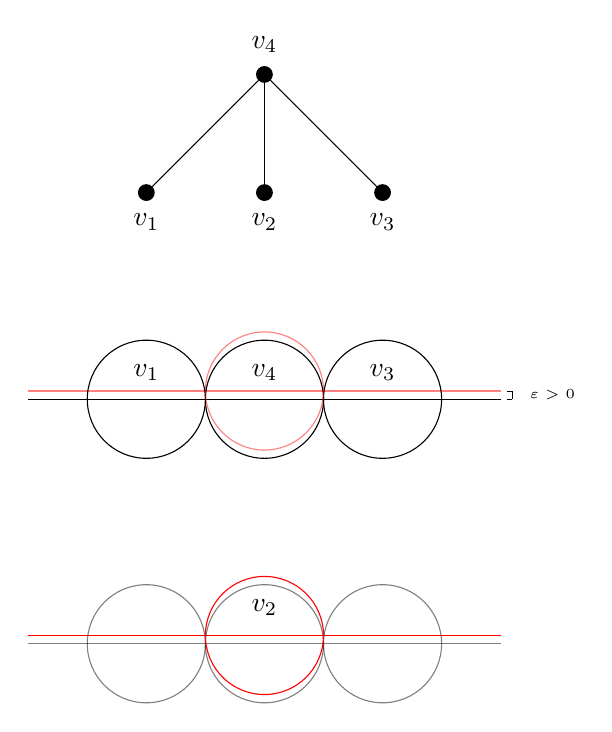
\begin{tikzpicture}[scale=1.5]

\draw (-2,0) -- (2,0);
\draw[red ,opacity = 0.5] (-2,0.07) -- (2,0.07);
\draw  (-1,0) circle [radius=0.5];
\draw[color=black] (-1,0.2265) node {$v_1$};
\draw  (0,0) circle [radius=0.5];
\draw[color=black] (0,0.2265) node {$v_4$};
\draw  (1,0) circle [radius=0.5];
\draw[color=black] (1,0.2265) node {$v_3$};

\draw[red, opacity = 0.5] (0,0.07) circle [radius=0.5];
\draw[color=black] (2.4386,0.0367) node {\tiny $\varepsilon > 0$};

% lines to describe distance (epsilon)
\draw[very thin] (2.1,0.07) -- (2.1,0);
\draw[very thin] (2.05,0.07) -- (2.1,0.07);
\draw[very thin] (2.05,0) -- (2.1,0);

\draw[opacity = 0.5] (-2,-2.07) -- (2,-2.07);
\draw[red] (-2,-2) -- (2,-2);
\draw[opacity = 0.5]  (0,-2.07) circle [radius=0.5];
\draw[opacity = 0.5]  (1,-2.07) circle [radius=0.5];
\draw[opacity = 0.5]  (-1,-2.07) circle [radius=0.5];
\draw[red] (0,-2) circle [radius=0.5];
\draw[color=black] (0,-1.765) node {$v_2$};

\node[draw,circle,inner sep=2pt,fill,label distance=1cm] (v1) at (0,2.75) {};
\draw[color=black] (0,3) node {$v_4$};
\node[draw,circle,inner sep=2pt,fill,label distance=1cm] (v3) at (0,1.75) {};
\draw[color=black] (0,1.5) node {$v_2$};
\node[draw,circle,inner sep=2pt,fill,label distance=1cm] (v2) at (-1,1.75) {};
\draw[color=black] (1,1.5) node {$v_3$};
\node[draw,circle,inner sep=2pt,fill,label distance=1cm] (v4) at (1,1.75) {};
\draw[color=black] (-1,1.5) node {$v_1$};
\draw  (v1) edge (v2);
\draw  (v1) edge (v3);
\draw  (v1) edge (v4);
\end{tikzpicture}
\end{scaletikzpicturetowidth}
\caption{A construction of $K_{1,3}$ with a disk realization, being this graph a TSG.}
\label{fig:thinK13}
\end{figure}

\begin{theorem}[Hayashi et al. \cite{hayashiThinStripGraphs2017}]
  There is no constant $t$ such that SG($t$) = TSG.
\end{theorem}

\begin{theorem}[Hayashi et al. \cite{hayashiThinStripGraphs2017}]
  There is no constant $t$ such that SG($t$) = UDG.
\end{theorem}

Hayashi et al. left some open problems. We try to expand the knowledge around some of these problems
to understand them better, largely for the recognition of this class of graphs. Before that, we see where this class lays in the hierarchy of classes. We know by definition that TSG $\subsetneq$ UDG.

\subsection{Interval graphs}

Thin strip graphs shares their geometrical structure with interval graphs (remember SG($0$) = UIG). In this subsection, we overview the results of Hayashi et al. \cite{hayashiThinStripGraphs2017} where they find maximal and minimal superclasses for TSG in the interval graphs presented in chapter \ref{chap:interval}. The following theorem will be proven by taking the proof written by Hayashi et al. in order to use their mapping in other theorems (e.g. \ref{chap:twolevel}).

\begin{theorem}[Hayashi et al. \cite{hayashiThinStripGraphs2017}]
  \label{theo:muigTSG}
  MUIG $\subsetneq$ TSG.
\end{theorem}

\proof{
First, we prove that MUIG $\neq$ TSG. This can be proven because $C_4 \in$ TSG if we take as points $(0,0),(0,\varepsilon),(1,0),(1,\varepsilon)$ with $1 >\varepsilon > 0$ and $C_4 \notin$ MUIG because it is a chordal graph.

Then, we have to prove that MUIG $\subseteq$ TSG. Let $G = (V,E) \in$ MUIG where each vertex is a unit mixed interval denoted as $I_v$. We define $t = \min\{|I_u\cap I_v| : |I_u\cap I_v| > 0, \{I_u,I_v\} \subseteq V\}$ and $s = \min\{\ell(I_v) - r(I_u) : \ell(I_v) > r(I_u), \{I_u,I_v\} \subseteq V\}$. We have then $t$ being the minimum length of an intersection bigger than zero (that is, not endpoint-adjacent) and $s$ is the minimum distance between non-adjacent vertices (also not endpoint-adjacent). We also define $c(I_v) = \frac{\ell(I_v) + r(I_v)}{2}$ as the center of the interval and $p(I_v) = (-1)^{\left \lfloor{c(I_v)}\right \rfloor }$.

Let $d$ be a real such that $0 < d < \frac{2}{3}$, $d\leq \frac{t}{4}$, $d < \frac{s}{2}$ and $\varepsilon \geq 2\sqrt{d-d^2}$. If we let $h = \sqrt{d-d^2}$, then we can create a $2h$-realization of $G$ with the following mapping:

\[ \phi(v) =
  \begin{cases}
      (c(I_v),0) & \text{if}\  I_v\  \text{is a closed interval} \\
      (c(I_v),hp(I_v)) & \text{if}\  I_v\  \text{is an open interval} \\
      (c(I_v)-d,hp(I_v)) & \text{if}\  I_v\  \text{is a closed-open interval} \\
      (c(I_v)+d,hp(I_v)) & \text{if}\  I_v\  \text{is an open-closed interval}
   \end{cases}
\]

For two vertices $u$ and $v$ of $G$ such that $u \leq v$, we have the three following cases:

\begin{enumerate}
  \item $r(I_u) < \ell(I_v)$:

    $I_u$ and $I_v$ are not adjacents, which means that $\text{dist}(\phi(u),\phi(v)) > 1$.
    If we minimize the distance between them we have $\phi(u) = (c(I_u)+d,hp(I_u))$ and $\phi(v) = (c(I_v)-d,hp(I_v))$ with $p(I_u) = p(I_v)$. Therefore, we only have to compare their $x$-coordinates:

    $$\text{dist}(\phi(u),\phi(v)) \geq (c(I_v)-d) - (c(I_u)+d) = c(I_v)-c(I_u) - 2d$$

    By definition, $s \leq l(I_v)-r(I_u)$. If we take the centers, then $s \leq c(I_v)-c(I_u) -1$, which means finally that $s +1 \leq c(I_v)-c(I_u)$

    $$\text{dist}(\phi(u),\phi(v)) \geq s + 1 - 2d > 1$$

  \item $r(I_u) > \ell(I_v)$:
    In this case $u$ and $v$ are adjacent. We maximize $\text{dist}(\phi(u),\phi(v))$ when $\phi(u) = (c(I_u)-d,hp(I_u))$ and $\phi(v) = (c(I_v)+d,hp(I_v))$ with $p(I_u) \neq p(I_v)$. Therefore,

\[    \begin{split}
    \text{dist}(\phi(u),\phi(v)) & \leq \sqrt{((c(I_v)+d)-(c(I_u)-d))^2 + (h+h)^2} \\
     & \text{with the same reasoning as before}\  c(I_v)-c(I_u) \leq 1-t\\
     & \leq \sqrt{(1-t+2d)^2 + 4h^2} \\
     & \leq \sqrt{(1-4d+2d)^2 + 4(d-d^2)} \\
     & = \sqrt{1-4d+4d^2 + 4d-4d^2} = 1
    \end{split}
\]

  \item $r(I_u) = \ell(I_v)$:

  In this case, $u$ and $v$ are adjacent only if $r(I_u)$ and $I_v$ are closed. We know that $c(I_v) = c(I_u)+1$ and $p(I_u) \neq p(I_v)$. Without loss of generality, we suppose that $p(I_u) = 1$ and $p(I_v) = -1$. We have two cases:
  \begin{enumerate}
    \item Both ends are closed. So we have this set of possible assignments for each one of the vertices:

    $$\phi(u) \in \{(c(I_u),0), (c(I_u)+d,h)\}$$
    $$\phi(v) \in \{(c(I_u)+1,0), (c(I_u)+1-d,-h)\}$$
    This gives us a rectangle with its diagonal smaller than one.

\item One of the ends is closed, we suppose $r(I_u)$ is open. In this case, we have these solutions:

  $$\phi(u) \in \{(c(I_u)-d,h), (c(I_u),h)\}$$
  $$\phi(v) \in \{(c(I_u)+1,0), (c(I_u)+1,-h), (c(I_u)+1\pm d,-h)\}$$

  Every distance between every points is greater than 1 if we take into consideration the domain of $d$. \qed

  \end{enumerate}
\end{enumerate}
}

From this theorem, UIG $\subsetneq$ TSG. Actually, there exists a stronger connection between these two classes:

\begin{theorem}[Breu \cite{breuAlgorithmicAspectsConstrained1996}]
  \label{theo:induced_TSG}
  Let $G$ a $c$-strip graph with $c \in \mathbb{R}_0^+$. $G$ has an induced $K_{1,3}$ or $C_4$ if and only if $G$ is not an unit interval graph.
\end{theorem}

Thin strip graphs can also be seen as unfettered unit interval graphs, which means that if a graph is a thin strip graph, then we can partition this graph with a level structure where each level is a clique. This information will be relevant in the next section.

\begin{theorem}[Hayashi et al. \cite{hayashiThinStripGraphs2017}]
  TSG $\subsetneq$ UUIG.
\end{theorem}

\proof{See \cite{hayashiThinStripGraphs2017}.}


\begin{figure}
\begin{center}
\begin{scaletikzpicturetowidth}{\textwidth}
\begin{tikzpicture}[scale=1]
  \node (0) [draw, rounded rectangle] {co-comparability graphs};
  \node (1) [below= of 0, draw, rounded rectangle] {unfettered unit interval graphs};
  \node (2) [below=of 1, draw, rounded rectangle] {thin strip graphs};
  \node (3) [below=of 2, draw, rounded rectangle] {mixed unit interval graphs};
  \node (4) [below=of 3, draw, rounded rectangle] {unit interval graphs};
  \node (5) [left=of 1, draw, rounded rectangle] {unit disk graphs};
  \node (6) [left=of 2, below=of 5] {};
  \draw[<-] (0) edge (1) (1) edge (2) (2) edge (3) (3) edge (4) (5) edge (6.south);
  \draw[-] (2) edge (6.south);

\end{tikzpicture}
\end{scaletikzpicturetowidth}
\end{center}
  \caption{Extension of the graph classes diagram from Figure \ref{fig:hierarchyTSG} with \emph{TSG} and \emph{UDG}.}
\label{fig:hierarchyTSG}
\end{figure}

\section{Characterization of thin strip graphs}

One of the main goals of this thesis is to characterize thin strip graphs by forbidden induced subgraphs. We know that TSG is an hereditary class, then a way to characterize this class of graphs is by looking for its forbidden subgraphs the same way as MUIG has been characterized by Joos. Furthermore, MUIG $\subsetneq$ TSG by Theorem \ref{theo:muigTSG}, so the first we can do is to check if the forbidden subgraphs of MUIG are also for TSG.


\subsection{Mixed unit interval graph forbidden subgraphs}

In the previous section we have shown that MUIG $\subsetneq$ TSG \ref{theo:muigTSG}. We have even shown every forbidden induced subgraph of MUIG in Chapter \ref{chap:interval}. Here we are going to overview these forbidden induced subgraphs and we their inclusion in TSG. Moreover, we will verify if one of these families is at least in UUIG.

In this subsection, we are going to see the relationship between thin strip graphs and mixed unit interval graphs.

\begin{figure}
\begin{center}
  \begin{scaletikzpicturetowidth}{\textwidth}
  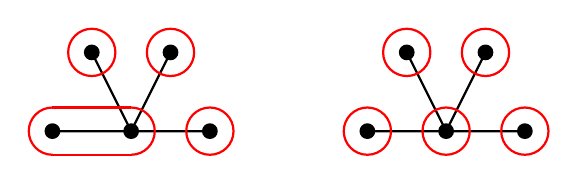
\begin{tikzpicture}[scale=1]
\def\ver{0.1} %size of a vertex
\def\x{1}

\def\xa{0.5}
\def\ya{0}

\def\xd{4.5}
\def\yd{0}


%graph R_0
\path[fill] (\xa+0.5,\ya) circle (\ver);
\path[fill] (\xa+1,\ya+1) circle (\ver);
\path[fill] (\xa+2,\ya+1) circle (\ver);
\path[fill] (\xa+2.5,\ya) circle (\ver);
\path[fill] (\xa+1.5,\ya) circle (\ver);

\draw[thick] (\xa+0.5,\ya)--(\xa+1.5,\ya)--(\xa+1,\ya+1)
(\xa+2,\ya+1)--(\xa+1.5,\ya)--(\xa+2.5,\ya);


\draw[thick,red] (\xa+2,\ya+1+ \ver+0.2) coordinate(a1)  arc (90:450:\ver +0.2) coordinate(a2);

\draw[thick,red] (\xa+1,\ya+1+ \ver+0.2) coordinate(d1)  arc (90:450:\ver +0.2) coordinate(d2);

\draw[thick,red] (\xa+2.5,\ya+ \ver+0.2) coordinate(e1)  arc (90:450:\ver +0.2) coordinate(e2);

\draw[thick,red] (\xa+0.5,\ya+ \ver+0.2) coordinate(b1)  arc (90:270:\ver +0.2) coordinate(b2);
\draw[thick,red] (\xa+1.5,\ya- \ver-0.2) coordinate(c1)  arc (270:450:\ver +0.2) coordinate(c2);

% reliate
\draw[thick,red] (c1) -- (b2) (c2)--(b1);

%graph R_0
\path[fill] (\xd+0.5,\yd) circle (\ver);
\path[fill] (\xd+1,\yd+1) circle (\ver);
\path[fill] (\xd+2,\yd+1) circle (\ver);
\path[fill] (\xd+2.5,\yd) circle (\ver);
\path[fill] (\xd+1.5,\yd) circle (\ver);

\draw[thick] (\xd+0.5,\yd)--(\xd+1.5,\yd)--(\xd+1,\yd+1)
(\xd+2,\yd+1)--(\xd+1.5,\yd)--(\xd+2.5,\yd);

\draw[thick,red] (\xd+2,\yd+1+ \ver+0.2) coordinate(a1)  arc (90:450:\ver +0.2) coordinate(a2);
\draw[thick,red] (\xd+1,\yd+1+ \ver+0.2) coordinate(d1)  arc (90:450:\ver +0.2) coordinate(d2);
\draw[thick,red] (\xd+2.5,\yd+ \ver+0.2) coordinate(e1)  arc (90:450:\ver +0.2) coordinate(e2);
\draw[thick,red] (\xd+1.5,\yd+ \ver+0.2) coordinate(d1)  arc (90:450:\ver +0.2) coordinate(d2);
\draw[thick,red] (\xd+0.5,\yd+ \ver+0.2) coordinate(e1)  arc (90:450:\ver +0.2) coordinate(e2);


\end{tikzpicture}
\end{scaletikzpicturetowidth}
\end{center}
\caption{Every possible clique partition of $R_0$. You may notice that any of the partitions is a level structure.}\label{fig:R0level}
\end{figure}

\begin{figure}[H]
\begin{center}
  \begin{scaletikzpicturetowidth}{\textwidth}
  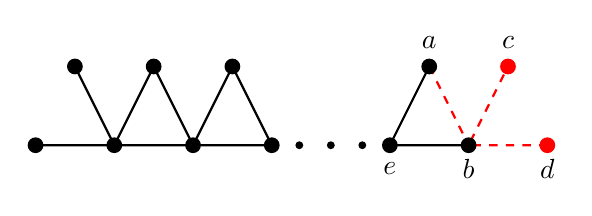
\begin{tikzpicture}[scale=1]
\def\ver{0.1} %size of a vertex
\def\x{1}

\def\xd{0}
\def\yd{0}

\draw[thick] (\xd,\yd)--(\xd+3,\yd)
(\xd+4.5,\yd)--(\xd+5.5,\yd)
(\xd+0.5,\yd+1)--(\xd+1,\yd)--(\xd+1.5,\yd+1)--(\xd+2,\yd)--(\xd+2.5,\yd+1)--(\xd+3,\yd)
(\xd+4.5,\yd)--(\xd+5,\yd+1);

\draw[thick, dashed, color=red] (\xd+6.5,\yd) -- (\xd+5.5,\yd)--(\xd+6,\yd+1) (\xd+5,\yd+1)--(\xd+5.5,\yd);

%graph R_i
\path[fill] (\xd,\yd) circle (\ver);
\path[fill] (\xd+1,\yd) circle (\ver);
\path[fill] (\xd+2,\yd) circle (\ver);
\path[fill] (\xd+3,\yd) circle (\ver);
\path[fill] (\xd+4.5,\yd) circle (\ver);
\path[fill] (\xd+5.5,\yd) circle (\ver);
\path[fill, color=red] (\xd+6.5,\yd) circle (\ver);
\path[fill] (\xd+0.5,\yd+1) circle (\ver);
\path[fill] (\xd+1.5,\yd+1) circle (\ver);
\path[fill] (\xd+2.5,\yd+1) circle (\ver);
\path[fill] (\xd+5,\yd+1) circle (\ver);
\path[fill, color=red] (\xd+6,\yd+1) circle (\ver);

\fill (\xd+3.35,\yd) circle (\ver/2);
\fill (\xd+3.75,\yd) circle (\ver/2);
\fill (\xd+4.15,\yd) circle (\ver/2);

\node (1) at (\xd+5.5,\yd-0.3) {$b$};
\node (2) at (\xd+6.5,\yd-0.3) {$d$};
\node (2) at (\xd+4.5,\yd-0.3) {$e$};
\node (4) at (\xd+5,\yd+1+0.3) {$a$};
\node (3) at (\xd+6,\yd+1+0.3) {$c$};

\end{tikzpicture}
\end{scaletikzpicturetowidth}
\end{center}
\caption{The graph $R_{i+1}$. You can see that the red edges and vertices are what differ from $R_i$.}\label{fig:ri+1}
\end{figure}

\begin{theorem}[Hayashi et al. \cite{hayashiThinStripGraphs2017}]
  $\mathcal{R}$ is a forbidden induced subgraph family of UUIG.
\end{theorem}

\begin{proof}
  We can prove this by induction on $i$.

  \begin{itemize}
    \item \emph{Case $i=0$}: $R_0 \notin$ UUIG because there is no clique partition of $R_0$ that is also a level structure as seen in Figure \ref{fig:R0level}.
    \item \emph{Case $i = i+1$}: We suppose that every valid clique partition of $R_i$ is not a level structure. See in Figure \ref{fig:ri+1} the edges and vertices that we add to generate $R_{i+1}$. We call $a,b$ the vertices that were disjoint in $R_i$ and $c,d$ the new vertices. These two vertices are adjacent to $b$.

    Let $\{b,c\}$ or $\{b,d\}$ be a level of our clique partition. By the hypothesis of induction we know that this is partition is not a level structure because this partition is a valid partition of $R_i$ because $a$ and $b$ are in different levels. The only way to create a new partition that is not a valid clique partition of $R_i$ is if $\{a,b\}$ is a level. In this case, however, the clique level $\{a,b\}$ will be adjacent to three cliques $\{c\}, \{d\}$ and $\{e, \dots\}$ so this clique partition is not a level structure either.
  \end{itemize}

  This proves that $R_i$ for every $i \in \mathbb{N}_0$ has not a clique level structure; thus, it is not an UUIG.
\end{proof}

We see that $\mathcal{R}$ is a family of forbidden subgraphs of TSG. Nevertheless, the rest of the forbidden subgraphs for MUIG are thin strip graphs. The main reason is because they are unfettered unit interval graphs. We see our first example with the forbidden graph for MUIG $F$.

\begin{figure}
\begin{center}
  \begin{scaletikzpicturetowidth}{\textwidth}
  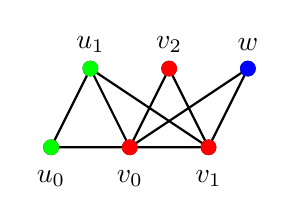
\begin{tikzpicture}[scale=1]
    \def\ver{0.1} %size of a vertex
    \def\x{1}

    \def\xa{0}
    \def\ya{0}

    %G_1
    \path[fill] (\xa+1,\ya) circle (\ver);
    \path[fill] (\xa+2,\ya) circle (\ver);
    \path[fill] (\xa+0.5,\ya+1) circle (\ver);
    \path[fill] (\xa+1.5,\ya+1) circle (\ver);
    \path[fill] (\xa+2.5,\ya+1) circle (\ver);
    \path[fill] (\xa,\ya) circle (\ver);

    \draw[thick] (\xa+1,\ya)--(\xa+2,\ya)
    (\xa+1,\ya)--(\xa+0.5,\ya+1)--(\xa+2,\ya)
    (\xa+1,\ya)--(\xa+2.5,\ya+1)--(\xa+2,\ya)
    (\xa+1,\ya)--(\xa+1.5,\ya+1)--(\xa+2,\ya)
    (\xa+1,\ya)--(\xa,\ya)--(\xa+0.5,\ya+1);

    \path[fill=red] (\xa+1,\ya) circle (\ver);
    \path[fill=red] (\xa+2,\ya) circle (\ver);
    \path[fill=green] (\xa+0.5,\ya+1) circle (\ver);
    \path[fill=red] (\xa+1.5,\ya+1) circle (\ver);
    \path[fill=blue] (\xa+2.5,\ya+1) circle (\ver);
    \path[fill=green] (\xa,\ya) circle (\ver);

    \node (1) at (\xa,\ya-0.4) {$u_0$};
    \node (1) at (\xa+0.5,\ya+1.3) {$u_1$};
    \node (1) at (\xa+1,\ya-0.4) {$v_0$};
    \node (1) at (\xa+2,\ya-0.4) {$v_1$};
    \node (1) at (\xa+1.5,\ya+1.3) {$v_2$};
    \node (1) at (\xa+2.5,\ya+1.3) {$w$};

\end{tikzpicture}
\end{scaletikzpicturetowidth}
\end{center}
\caption{The graph $F$ where each level is represented by a different color.}\label{fig:graphF_clique}
\end{figure}

\begin{figure}[t]
\begin{center}
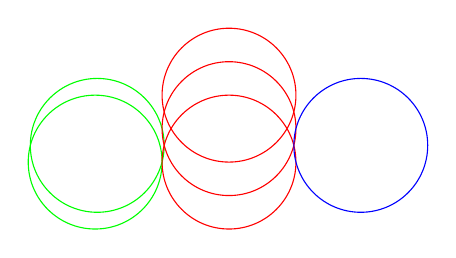
\begin{tikzpicture}[scale=1.7]

\def\ver{0.5}
\def\verp{0.04} %size of a vertex
\def\epsilon{0.5}


\draw[color=green] ({((\epsilon/4)*(\epsilon/4) - 1)*2*\ver},{(\epsilon/4)*2*\ver}) circle (\ver);
\draw[color=green] (-1,0) circle (\ver);

\draw[color=red] (0,0) circle (\ver);
\draw[color=red] (0,{(\epsilon / 2) *2* \ver}) circle (\ver);
\draw[color=red] (0,{(2* \epsilon / 2)*2* \ver}) circle (\ver);

\draw[color=blue] ({(1 - (\epsilon/4)*(\epsilon/4))*2*\ver},{(\epsilon/4)*2*\ver}) circle (\ver);


\end{tikzpicture}
\end{center}
\caption{Realization of $F$ as a thin strip graph.}\label{fig:graphF_thin}
\end{figure}

\begin{theorem}
  $F \in$ TSG.
\end{theorem}

\proof{
To prove this we have to find an $\varepsilon$-realization for our graph $F = (V,E)$ with $\varepsilon$ arbitrarily small. Let $\phi(v)$ be the mapping of our vertices on the plane. $F$ has a level structure $L = \{\{u_0, u_1\}, \{v_0, v_1, v_2\}, \{w\}\}$ as shown in Figure \ref{fig:graphF_clique}.

We begin to construct the representation as a thin strip graph by placing the vertices $v_0, v_1, v_2$ on the plane. Simply, we place them on the same $x$ coordinate with an equal distance from $v_0$ to $v_1$ and $v_1$ to $v_2$ such that they are all adjacent, being those on a $y$ coordinate smaller than $\varepsilon$:

$$\phi(v_k) = \Bigg(0, \varepsilon \frac{k}{2}\Bigg)$$

for $k \in \{0,1,2\}$.\\

We continue with $w$; $w$ has to be adjacent to $v_0$ and $v_1$, but not $v_2$. We pursue to place it on a $y$ coordinate that is located in the middle between $0$ and $\frac{\varepsilon}{2}$ (the $y$ coordinates of $v_0$ and $v_1$), which is $\frac{\varepsilon}{4}$. Now we have to find a $x$ coordinate for $w$ such that it touches both $v_0$ and $v_1$ but does not intersect with $v_2$. By symmetry, we only have to check the adjacency of $v_0$ and $v_2$. We can calculate a point such that the distance between $w$ and $v_0$ equals one:

\begin{equation*}
  \begin{split}
    \sqrt{\phi(w)_y^2 + \Big(\frac{\varepsilon}{4}\Big)^2} &= 1\\
    \phi(w)_x^2 + \Big(\frac{\varepsilon}{4}\Big)^2 &= 1\\
    \phi(w)_x^2 &= 1 - \Big(\frac{\varepsilon}{4}\Big)^2\\
    \phi(w)_x &= \sqrt{1 - \Big(\frac{\varepsilon}{4}\Big)^2}\\
    \phi(w)_x &= \sqrt{\frac{16 - \varepsilon^2}{16}}\\
    \phi(w)_x &= \frac{\sqrt{16 - \varepsilon^2}}{4}\\
  \end{split}
\end{equation*}

and by symmetry, $-\frac{\sqrt{16 - \varepsilon^2}}{4}$ is also a candidate. We only have to see if it touches $v_2$ for every $\varepsilon$:

\begin{equation*}
  \begin{split}
    \sqrt{\Bigg(\frac{\sqrt{16 - \varepsilon^2}}{4}\Bigg)^2 + \varepsilon^2} &> 1\\
    \sqrt{\frac{16 - \varepsilon^2}{16} + \varepsilon^2} &> 1\\
    \sqrt{\frac{16 - \varepsilon^2 + 16\varepsilon}{16}} &> 1\\
    \sqrt{\frac{16 + 15\varepsilon^2}{16}} &> 1\\
    \frac{1}{4}\sqrt{16 + 15\varepsilon^2} &> 1\\
  \end{split}
\end{equation*}

the expression of the left will always be bigger than one if $\varepsilon \neq 0$, which means that $w$ will never be adjacent to $v_2$.

$$\phi(w) = \Bigg(\frac{\sqrt{16 - \varepsilon^2}}{4}, \frac{\varepsilon}{4}\Bigg)$$

Finally, we have to place $u_0, u_1$. We can remark that the neighbours of $u_1$ in the second level correspond to the neighbours of $w$ , so it will be placed symmetrically with respect to 0 with the same $y$ coordinate, as we have proven before. Finally, $u_0$ has to be adjacent to $v_0$. We can place it at $(-1,0)$ with the same argument as the construction of $K_{1,3}$ (see Figure \ref{fig:thinK13}). The other vertices of the second level $v_1$ and $v_2$ will not be adjacent to $u_0$ unless their $y$ coordinate is 0, which is not the case.

$$\phi(u_1) = \Bigg(-\frac{\sqrt{16 - \varepsilon^2}}{4}, \frac{\varepsilon}{4}\Bigg)$$
$$\phi(u_2) = (-1, 0)$$

You can find a visual representation of this graph in Figure \ref{fig:graphF_thin}. \qed
}


\begin{figure}[t]
\begin{center}
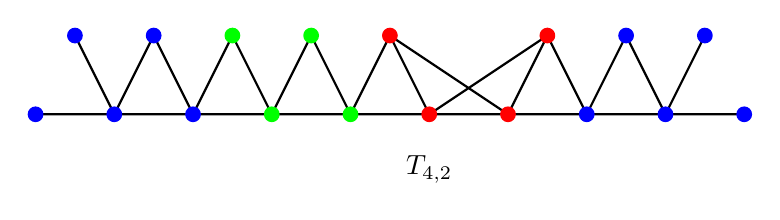
\begin{tikzpicture}[scale=1]
\def\ver{0.1} %size of a vertex
\def\x{1}

\def\xa{0}
\def\ya{0}

\def\xb{4}
\def\yb{0}

\def\xc{9}
\def\yc{0}

\def\xd{3}
\def\yd{-2.5}

\draw[thick] (\xc-2,\yc)--(\xc+7,\yc)
(\xc-1.5,\yc+1)--(\xc-1,\yc)--(\xc-0.5,\yc+1)--(\xc,\yc)--(\xc+0.5,\yc+1)--(\xc+1,\yc)--(\xc+1.5,\yc+1)--(\xc+2,\yc)--(\xc+2.5,\yc+1)--(\xc+3,\yc)--(\xc+4.5,\yc+1)
(\xc+5.5,\yc+1)--(\xc+5,\yc)--(\xc+4.5,\yc+1)--(\xc+4,\yc)--(\xc+2.5,\yc+1)
(\xc+5.5,\yc+1)--(\xc+6,\yc)--(\xc+6.5,\yc+1);

%graph T_{2,1}
\path[fill=blue] (\xc-2,\yc) circle (\ver);
\path[fill=blue] (\xc-1,\yc) circle (\ver);
\path[fill=blue] (\xc,\yc) circle (\ver);
\path[fill=green] (\xc+1,\yc) circle (\ver);
\path[fill=green] (\xc+2,\yc) circle (\ver);
\path[fill=red] (\xc+3,\yc) circle (\ver);
\path[fill=red] (\xc+4,\yc) circle (\ver);
\path[fill=blue] (\xc+5,\yc) circle (\ver);
\path[fill=blue] (\xc+6,\yc) circle (\ver);
\path[fill=blue] (\xc+7,\yc) circle (\ver);

\path[fill=blue] (\xc-1.5,\yc+1) circle (\ver);
\path[fill=blue] (\xc-0.5,\yc+1) circle (\ver);
\path[fill=green] (\xc+0.5,\yc+1) circle (\ver);
\path[fill=green] (\xc+1.5,\yc+1) circle (\ver);
\path[fill=red] (\xc+2.5,\yc+1) circle (\ver);
\path[fill=red] (\xc+4.5,\yc+1) circle (\ver);
\path[fill=blue] (\xc+5.5,\yc+1) circle (\ver);
\path[fill=blue] (\xc+6.5,\yc+1) circle (\ver);

\node (1) at (\xc+3,\yc-0.7) {$T_{4,2}$};

\end{tikzpicture}
\end{center}
\caption{The graph $T_{4,2}$ with the diamond in red and the arms in green. The $K_{1,3}$ bis from previous lemma is in blue.}\label{fig:graph_T_clique}
\end{figure}

\begin{figure}[t]
\begin{center}
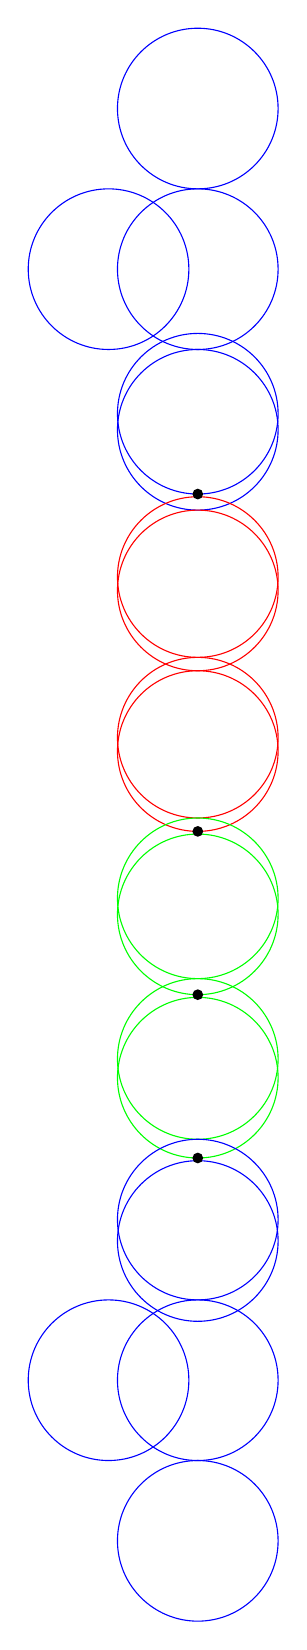
\begin{tikzpicture}[rotate=90, scale=1.7]

\def\ver{0.6}
\def\verp{0.04} %size of a vertex

\draw[color=blue] (\ver*4-0.1,0) circle (\ver);
\draw[color=blue] (\ver*4-0.1+0.12,0) circle (\ver);
\draw[color=blue] (\ver*6-0.1,0) circle (\ver);
\draw[color=blue] (\ver*6-0.1,\ver+\ver/9) circle (\ver);
\draw[color=blue] (\ver*8-0.1,0) circle (\ver);

\draw[color=red] (0,0) circle (\ver);
\draw[color=red] (\ver*2-0.1,0) circle (\ver);
\draw[color=red] (\ver*2,0) circle (\ver);
\draw[color=red] (-0.1,0) circle (\ver);
\draw[color=green] (-\ver*2,0) circle (\ver);
\draw[color=green] (-\ver*2-0.12,0) circle (\ver);
\draw[color=green] (-\ver*4,0) circle (\ver);
\draw[color=green] (-\ver*4-0.14,0) circle (\ver);
\draw[color=blue] (-\ver*6,0) circle (\ver);
\draw[color=blue] (-\ver*6-0.16,0) circle (\ver);
\draw[color=blue] (-\ver*8,0) circle (\ver);
\draw[color=blue] (-\ver*8,\ver+\ver/9) circle (\ver);
\draw[color=blue] (-\ver*10,0) circle (\ver);

\path[fill] (\ver*3+0.02,0) circle (\verp);
\path[fill] (-\ver-0.1,0) circle (\verp);
\path[fill] (-\ver*3-0.12,0) circle (\verp);
\path[fill] (-\ver*5-0.14,0) circle (\verp);

\end{tikzpicture}
\end{center}
\caption{A realization as a thin strip graph of $T_{4,2}$ from Figure \ref{fig:graph_T_clique}. The distance between the disks disminishes with the value of $\varepsilon$, but the disks designated by the black points will never touch.}
\end{figure}

\todo[inline]{Add drawings for $S$ and $S''$ like Figure \ref{fig:graph_T_clique} and the actual proofs (similar to proof of $F$, only have to write them!).}


\section{Recognition}

The recognition of this class of graphs is approached by Breu in his thesis \cite{breuAlgorithmicAspectsConstrained1996}. He gives a polynomial-time algorithm to recognise strip graphs for a given input with an assignment of $y$-coordinates for each vertex of the graph and an orientation of the edges of its complement.

\begin{theorem}[Breu \cite{breuAlgorithmicAspectsConstrained1996}]
  Let $G = (V,E,\gamma,\overrightarrow{E})$ a graph where $\gamma: V \to [0,c]$ is a function associating a $y$-coordinate (or a level) to each vertex and $\overrightarrow{E}$ an orientation of the complement of the graph. The recognition of $c$-strip graphs with this input is in $\mathcal{P}$.
\end{theorem}

\begin{obs}
  Recognition of $c$-strip graphs without a given $\overrightarrow{E}$ is in $\mathcal{NP}$.
\end{obs}

\proof{
  Given an polynomial-time algorithm with a complexity of $O(f(n))$ to solve recognition of $G = (V,E,\gamma,\overrightarrow{E})$, we can run again this algorithm by testing every possible orientation of its complement. This algorithm would take $O(f(n))2^{|E|-1} = O(f(n)2^{|E|})$ time to execute. \qed
}\\

We would like to have an algorithm that solves this problem without knowing the $y$-coordinates of the vertices. Nevertheless, further research would concentrate on recognition of UUIGs. We know that TSG $\subsetneq$ UUIG, and recognition of UUIGs is $\mathcal{NP}$. If we the problem of recognising TSG given a UUIG and is solved in polynomial time, then TSG recognition would be $\mathcal{NP}$. However, given the observations in the end of chapter \ref{chap:interval}, there may be a polynomial-time algorithm for UUIG.
